\documentclass[oneside, final, 11pt]{article}
\usepackage[utf8]{inputenc}
\usepackage[T2A]{fontenc}
\usepackage[russian]{babel}
\usepackage{natbib}
\usepackage{graphicx}
\usepackage{amsmath}
\usepackage{xcolor}
\usepackage{amssymb}
\usepackage{graphicx}
\graphicspath{ {images/} }
\usepackage{subcaption}

\usepackage[paper=a4paper, margin=2cm, bottom=2cm]{geometry}

\newcommand\tab[1][1cm]{\hspace*{#1}}

\begin{document}
\begin{titlepage}
\newgeometry{margin=1cm}

\centerline{\large \bf МИНИСТЕРСТВО ОБРАЗОВАНИЯ РЕСПУБЛИКИ БЕЛАРУСЬ}
\bigskip
\bigskip
\centerline{\large \bf БЕЛОРУССКИЙ ГОСУДАРСТВЕННЫЙ УНИВЕРСИТЕТ}
\bigskip
\bigskip
\centerline{\large \bf ФАКУЛЬТЕТ ПРИКЛАДНОЙ МАТЕМАТИКИ И ИНФОРМАТИКИ}
\vfill
\vfill
\vfill
\centerline{\large \bf МЕТОДЫ ЧИСЛЕННОГО АНАЛИЗА}
\bigskip
\bigskip
\vfill
\begin{centering}
  \large Лабараторная работа №1 \\
 ``Численное решение задачи Коши для ОДУ'' \\
  студента 3 курса 1 группы \\
  \bf Пажитных Ивана Павловича \\
\end{centering}
\vfill
\vfill
\hfill
\begin{minipage}{0.25\textwidth}
  {\large{\bf Преподаватель} \\
{\it Бондарь Иван \\ Васильевич}}
\end{minipage}
\vfill
\vfill
\centerline{\large \bf Минск 2016}

\end{titlepage}

\restoregeometry

\section{Условие}
Написать программу, реализующую метод, указанный в варианте с автоматическим выбором шага интегрирования (используя правило Рунге). Экспериментально сравнить эффективность использованного метода с явным методом Эйлера.\\ \\
Результаты оформить в виде отчета, в который включить графики компонент численного решения. Кроме того, включить в отчет результаты сравнения используемых методов, оформленные в виде таблицы (провести численные эксперименты с точностью $tol = 0.000001$)\\

Входные данные:
\begin{itemize}
    \item $tol$ - требуемая точность
    \item $h_0$ - величина начального шага
    \item $T$ - конечная точка интегрирования
\end{itemize}

Выходные данные:
\begin{itemize}
    \item $N_{tot}$ - общее количество шагов по времени
    \item $N_A$ - количество принятых шагов
    \item $N_R$ - количество отброшенных шагов
    \item $t$ - время работы программы
\end{itemize}


\section{Вариант}
\begin{center}
    \bf №4. ``Аттрактор Лоренца''
\end{center}

Данная система ОДУ появилась в результате попыток математического моделирования климата. При определённом выборе параметров траектория любого решения этой системы стремится при $t \rightarrow \infty$ к асимптотически устойчивому непериодическому решению — так называемому «странному аттрактору».

\begin{equation}
    \begin{cases}
    y'_1 = -\sigma(y_1 - y_2) \\
    y'_2 = -y_1 y_3 + r y_1 - y_2\\
    y'_3 = y_1 y_2 - b y_3 \\
    \end{cases}
\end{equation}
\begin{equation}
    y_0 = (-8,8,r-1)^T
\end{equation}

Упомянутое хаотичное поведение решения достигается, например, при следующих значениях параметров:
\begin{equation}
    \sigma = 10, b = \frac{8}{3}, r = 28
\end{equation}

Решить явным методом Рунге-Кутты 4-го порядка.

\section{Теория}

\subsection{Явный метод Эйлера}
\begin{equation}
    \begin{cases}
    x_i = x_{i-1} + h, \\
    f(x_i, y_i) = y'(x_i), \\
    y_i = y_{i-1} + h f(x_{i-1}, y_{i-1}), \\
    i=\overline{1,n}
    \end{cases}
\end{equation}

\subsection{Явный метод Рунге-Кутты 4-го порядка}
\begin{equation}
\begin{tabular}{c|c|c|c|c}
    0           &   &   &   &                   \\\hline
$\frac{1}{2}$   & $\frac{1}{2}$  &   &   &      \\\hline
$\frac{1}{2}$   & 0  & $\frac{1}{2}$  &   &     \\\hline
    1           & 0  & 0  & 1  &                \\\hline
                & $\frac{1}{6}$ & $\frac{2}{6}$ & $\frac{2}{6}$ & $\frac{1}{6}$\\
\end{tabular}
\end{equation}

Подставляя коэффициенты:
\begin{equation}
    \begin{cases}
    k_1 = f(x_i, y_i) \\
    k_2 = f(x_i + \frac{1}{2} h, y_i + \frac{1}{2} k_1 h) \\
    k_3 = f(x_i + \frac{1}{2} h, y_i + \frac{1}{2} k_2 h) \\
    k_4 = f(x_i + h, y_i + k_3 h) \\
    \end{cases}
\end{equation}

\begin{equation}
y_i = y_{i-1} + ( \frac{1}{6} k_1 + \frac{2}{6} k_2 + \frac{2}{6} k_3 + \frac{1}{6} k_4) h, i=\overline{1,n}
\end{equation}

\subsection{Правило Рунге}
Для оценки требуется решить задачу на 2 сетках: две итерации с шагом h ($y_1$, $y_2$)  и одна — с шагом 2h ($\overline{y_2}$), получаем оценку:

\begin{equation}
\varepsilon_i = \frac{y_2-\overline{y_2}}{2^p-1}
\end{equation}

При подборе следующий шаг считается как $h_{new}<\delta h$, где $\delta$:

\begin{equation}
\delta = \left(\frac{tol}{|\varepsilon|}\right)^{\frac{1}{p+1}}
\end{equation}

\section{Отчет}
\subsection{$y(0)=(-8, -8, 27)$}
\begin{tabular}{|c|c|c|c|c|c|}
\hline
tol     &   Метод       &   h   &   n   &   N   &   t   \\\hline
1e-07   &   Эйлера      &   4.92014936374e-06   &   203245   &   2   &   0.96827507019s   \\\hline
1e-07   &   Рунге-Кутта &   0.00222565354887   &   449   &   2   &   0.0159111022949s   \\\hline
\end{tabular} \\ \\
где $n$ - кол-во итераций последнего вычисления для шага h, \\
$N$ - кол-во пересчётов шага $h$, для отрезка интегрирования $[0, 1]$, для начально шага $h_0=0.1$ \\
$y_n = [9.05401908\tab14.55586445\tab18.40818043]$ - методом Эйлера \\
$y_n = [9.01971044\tab14.50963827\tab18.35917819]$ - методом Рунге-Кутта \\

\subsection{$y(0)=(10, 1, 27)$}
\begin{tabular}{|c|c|c|c|c|c|}
\hline
tol     &   Метод       &   h   &   n   &   N   &   t   \\\hline
1e-07   &   Эйлера      &   8.0230021755e-06   &   124641   &   2   &   0.586709022522s   \\\hline
1e-07   &   Рунге-Кутта &   0.00361778866086   &   276   &   2   &   0.0107769966125s   \\\hline
\end{tabular} \\ \\
где $n$ - кол-во итераций последнего вычисления для шага h, \\
$N$ - кол-во пересчётов шага $h$, для отрезка интегрирования $[0, 1]$, для начально шага $h_0=0.1$ \\
$y_n = [8.06618792\tab12.49772564\tab18.73044515]$ - методом Эйлера \\
$y_n = [8.00373455\tab12.40821836\tab18.66281849]$ - методом Рунге-Кутта \\

\begin{figure}[h]
    \centering
    \begin{subfigure}[h]{0.45\textwidth}
        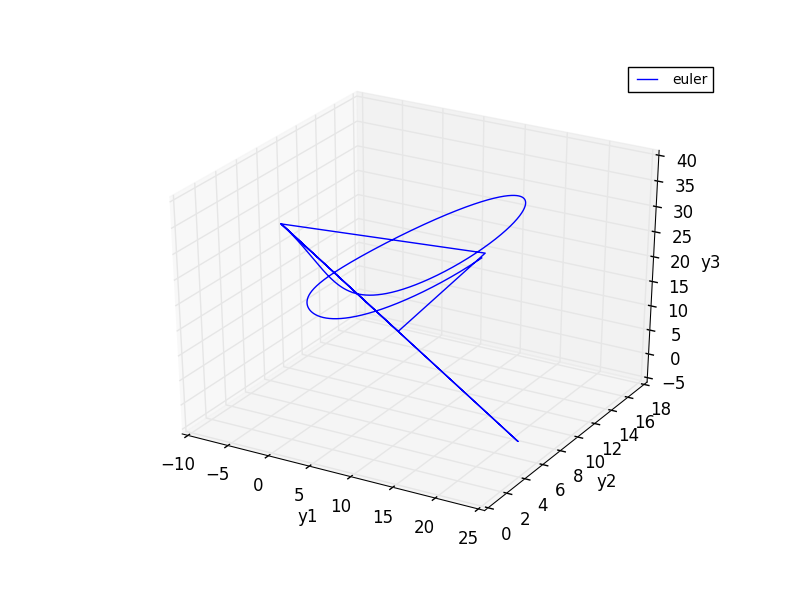
\includegraphics[width=\textwidth]{figure_2.png}
        \caption{Эйлера}
        \label{s1}
    \end{subfigure}
    ~
    \begin{subfigure}[h]{0.45\textwidth}
        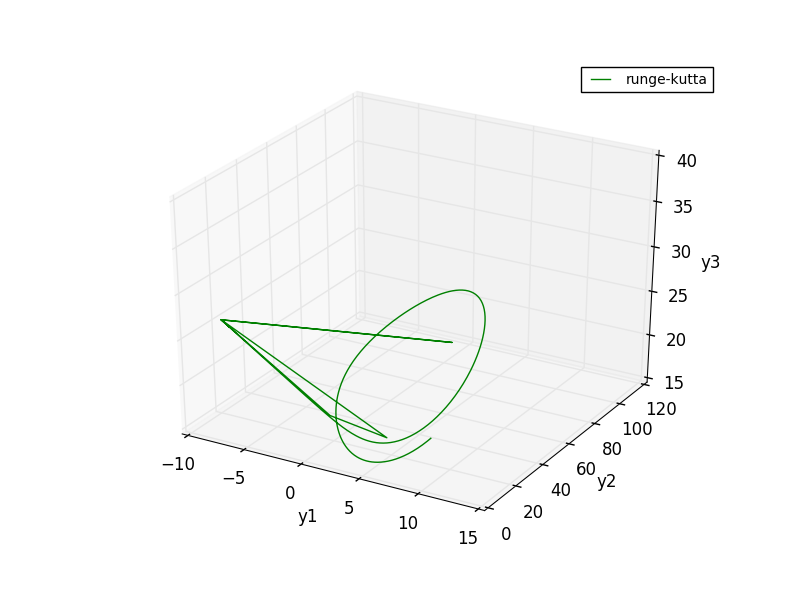
\includegraphics[width=\textwidth]{figure_3.png}
        \caption{Рунге-Кутты}
        \label{s2}
    \end{subfigure}
     ~
    \begin{subfigure}[h]{1\textwidth}
        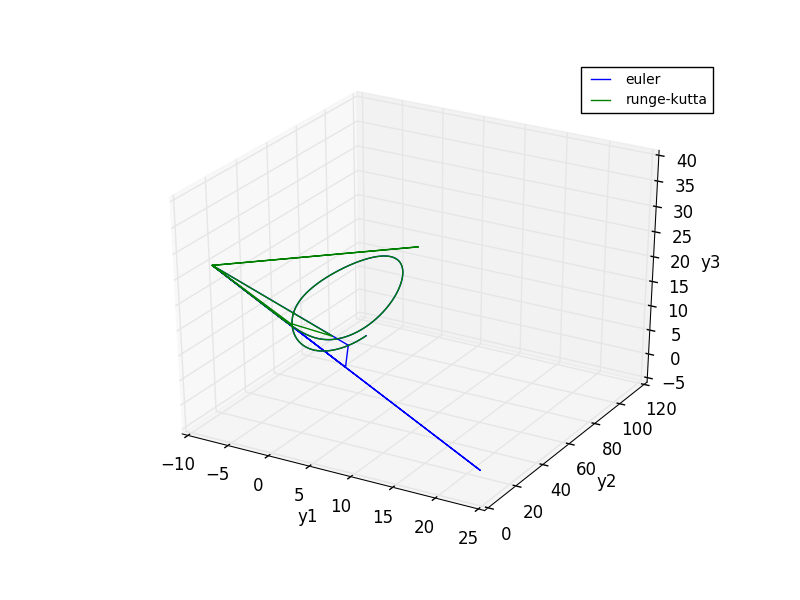
\includegraphics[width=\textwidth]{figure_1.png}
        \caption{совместный}
        \label{s2}
    \end{subfigure}
    \caption{Графики решения для 4.1}
\end{figure}

\begin{figure}[h]
    \centering
    \begin{subfigure}[h]{0.45\textwidth}
        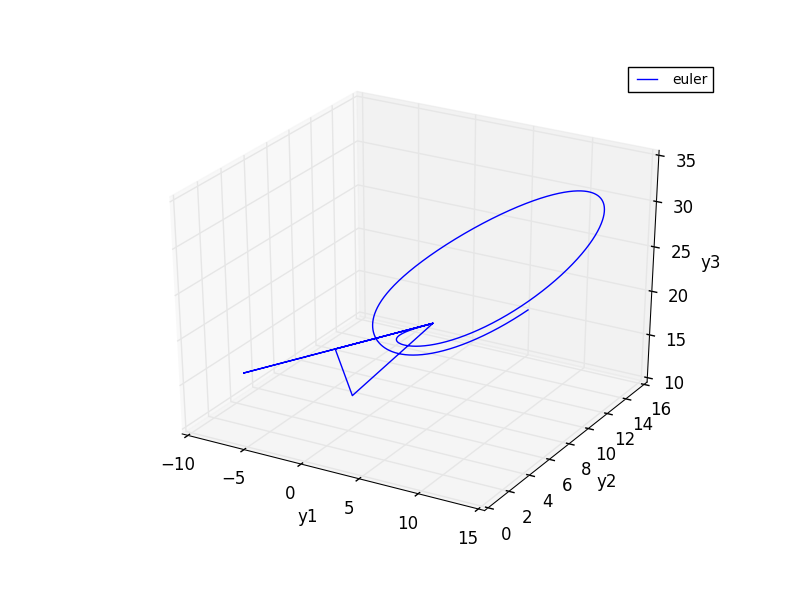
\includegraphics[width=\textwidth]{figure_5.png}
        \caption{Эйлера}
        \label{s1}
    \end{subfigure}
    ~
    \begin{subfigure}[h]{0.45\textwidth}
        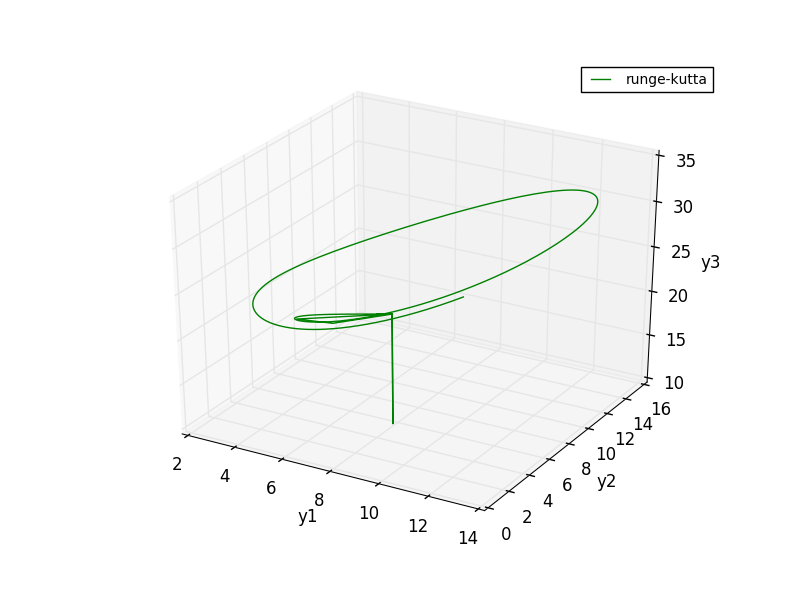
\includegraphics[width=\textwidth]{figure_6.png}
        \caption{Рунге-Кутты}
        \label{s2}
    \end{subfigure}
     ~
    \begin{subfigure}[h]{1\textwidth}
        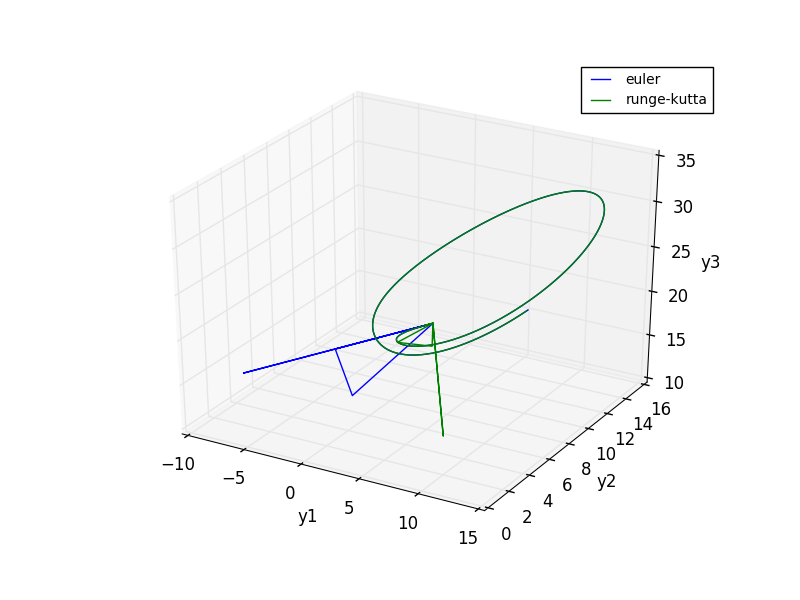
\includegraphics[width=\textwidth]{figure_4.png}
        \caption{совместный}
        \label{s2}
    \end{subfigure}
    \caption{Графики решения для 4.2}
\end{figure}

\end{document}